\documentclass [a4paper, 12pt]{article}

\usepackage[utf8]{inputenc}
\usepackage{amssymb}
\usepackage{amsmath}
\usepackage{bm}
\usepackage{epsfig}
\usepackage{graphicx}
\usepackage{times}
\usepackage{float}
\usepackage[usenames,dvipsnames]{color}
\usepackage{caption}
\usepackage{subcaption}
\usepackage{hyperref}
\usepackage{cleveref}

\textwidth 16 cm
\textheight 23 cm
\setlength{\oddsidemargin}{0.1 cm}
\setlength{\topmargin}{1 cm}
\setlength{\headheight}{0cm}
\setlength{\headsep}{0cm}
\setlength{\footskip}{0.75cm}
\setlength{\parindent}{0cm}
\setlength{\oddsidemargin}{0.1 cm}
\setlength{\itemsep}{10pt}
\bibliographystyle{gcs}

\DeclareUnicodeCharacter{2212}{-}
\newcommand{\matr}[1]{\bm{#1}}  

\begin{document}
 
\begin{figure}[H]
\begin{center}
  
\includegraphics[scale=0.45]{Figures/GCS-hlrs-fzj-lrz.jpg}\\
\end{center}
\end{figure}

\begin{center}
{\LARGE \bf Project Proposal for Tier0/Tier1 HPC Access} \\

\bigskip
\bigskip
\bigskip
\end{center}
\textbf{Period}\\
\phantom{MM}\textit{01.11.2017-31.10.2018}

\bigskip
\textbf{Project title}\\
\phantom{MM}\textit{KKRnano: Quantum description of skyrmions in chiral B20 magnets}

\bigskip
\textbf{Type of project}\\
\phantom{MM} \textit{new project}

%\bigskip
%\textbf{Project ID}\\
%\phantom{MM} \textit{Please provide in case of a project extension}

\bigskip
\textbf{Principal investigator}\\
\phantom{MM} \textit{ Prof. Dr. Stefan Bl{\"u}gel,
Institute for Advanced Simulation and Peter Gr\"unberg Institut, Forschungszentrum J\"ulich, D-52425 J\"ulich, Germany
}

\bigskip
\textbf{Project contributor(s)}\\

\phantom{MM} \textit{Marcel Bornemann,
Institute for Advanced Simulation and Peter Gr\"unberg Institut, Forschungszentrum J\"ulich, D-52425 J\"ulich, Germany
}

\phantom{MM} \textit{Dr. Sergii Grytsiuk,
Institute for Advanced Simulation and Peter Gr\"unberg Institut, Forschungszentrum J\"ulich, D-52425 J\"ulich, Germany
}

\phantom{MM} \textit{Dr. Roman Kovacik,
Institute for Advanced Simulation and Peter Gr\"unberg Institut, Forschungszentrum J\"ulich, D-52425 J\"ulich, Germany
}


\phantom{MM} \textit{Dr. Rudolf Zeller,
Institute for Advanced Simulation and Peter Gr\"unberg Institut, Forschungszentrum J\"ulich, D-52425 J\"ulich, Germany
}

\phantom{MM} \textit{Dr. Phivos Mavropoulos,
Institute for Advanced Simulation and Peter Gr\"unberg Institut, Forschungszentrum J\"ulich, D-52425 J\"ulich, Germany
}

\phantom{MM} \textit{Dr. Paul F. Baumeister,
Institute for Advanced Simulation and J\"ulich Supercomputing Centre, Forschungszentrum J\"ulich, D-52425 J\"ulich, Germany
}


\newpage

\vfill
\tableofcontents
\vfill

\newpage



\section{Introduction}
\rule{\textwidth}{0.4pt}\\
\textit{Give a short outline of the scientific background of your research, including references.}\\

\textit{(about 1 page)}

We have developed a unique electronic structure code, 
KKRnano \cite{zeller_towards_2008,thiess_massively_2012},
specifically designed for petaFLOP computing. Our method scales linearly
with the number of atoms, so that we can realize system sizes of up to 
458752 atoms in a unit cell. This has already been shown on the full JUQUEEN
machine \cite{brommel_juqueen_2017}.
\\
Recently, we implemented a relativistic generalization of our algorithm 
enabling us to calculate complex non-collinear magnetic structures, such as skyrmions,
in real space. Skyrmions are two-dimensional magnetization solitons, i.e. two-dimensional
magnetic structures localized in space, topologically protected by a non-trivial
magnetization texture, which has particle-like properties. 
These days, they constitute one of the most active subjects in the field of 
magnetism, because such topological solitons are considered to be the smallest 
information-carrying particles at room temperature \cite{fert_skyrmions_2013,castelvecchi_strange_2017}. 
\\
We plan to perform large-scale density functional theory (DFT) calculations with 
KKRnano for materials exhibiting these complex magnetic skyrmion textures. We would like to use Hazel Hen
because test runs showed that KKRnano performs best on machines with Sandy Bridge
architecture.
The focus of our work is on the germanide MnGe, as it exhibits a three-dimensional magnetic structure
that is not yet understood (see preliminary results
\cite{tanigaki_real-space_2015,rybakov_new_2016,bornemann_investigation_2017}).



\section{Preliminary Work}
\rule{\textwidth}{0.4pt}\\
\textit{Provide a brief summary of your preliminary work in connection with the proposed project, including references.}\\

\textit{(about 1 to 2 pages)}

It is fair to state that our group has accumulated strong expertise
in the field of magnetism\cite{bode_chiral_2007,heinze_spontaneous_2011,brede_long-range_2014,
dupe_engineering_2016,gayles_dzyaloshinskii-moriya_2015}
\\
The code KKRnano was first applied to Gd doped GaN, where special emphasis was placed on
magnetic interactions between defects \cite{thiess_superparamagnetism_2012}. Subsequently,
the phase change material GeSbTe was investigated \cite{zhang_role_2012}.
\\
During the last two years we have completely rewritten the code and considerably improved 
its flexibility with respect to the number of cores and the number of MPI tasks and
OpenMP threads that can be used in production runs. By changing the computational algorithms
we have also improved the computational efficiency both for conventional
supercomputers (e.g. JUQUEEN) and the cluster-booster architecture
(e.g. NVIDIA Tesla GPUs) \cite{dutot_addressing_2016}.
In the latest versions of KKRnano BLAS routines for linear algebra are used throughout the code
enhancing both readability and performance of the code. Furthermore, KKRnano is now
fully FORTRAN90 compliant with all the subroutines embedded in modules.
In order to benefit from accelerators installed in current and upcoming machines we
ported the core part of KKRnano, i.e. the TFQMR solver, to GPUs. The TFQMR solver was rewritten
in C++ and utilizes cuBLAS routines from the CUDA toolkit developed by NVIDIA.
\\
Subsequently, we tested the new version of the code for several large systems, 
in particular for MnGe supercells with B20 structure containing between 8192 and 458752 atoms,
during the JUQUEEN Extreme Scaling Workshop 2017 \cite{brommel_juqueen_2017}.
Due to limited computing time test runs for B20-MnGe were conducted on a smaller scale on JURECA and Hazel Hen.
As expected, performance results are similar for both machines and superior to JUQUEEN.
The results obtained within the test project on Hazel Hen (ACID 44110) entered
in our estimate of computational costs in \cref{sec:just}.
\\
As a first step towards a comprehensive understanding of skyrmionic textures in B20-MnGe we
performed simulations based on simple micromagnetic models that can provide an elementary understanding
of magnetism in many-body systems. A more detailed explanation of our results is given in \cref{sec:desc}.
\\
Additionally, the elementary unit cell consisting of 8 atoms (4 Mn and 4 Ge) was
studied with KKRnano to get a feeling of how parameters should be chosen and
to ensure that quantities obtained from DFT
match those observed in experiment.
Our calculations yielded an equilibrium lattice constant that is within the tolerance limit
associated with local density approximation as well as a magnetic moment that is reasonably close to
the one
found in experiment.



\section{Description of the Project}
\label{sec:desc}
\rule{\textwidth}{0.4pt}\\
\subsection{Project Details}
%\textit{Describe your research project in detail, structured in sub-projects, if applicable. Include discussion of the scientific questions that you are planning to address and the overall scientific goals of the project. It is important that you describe the innovative aspects, impact and topicality of the proposal.}
%\begin{itshape}
%\begin{itemize}\setlength{\itemsep}{-2pt}
%  \item Scientific questions you want to address
%  \item Scientific objectives
%  \item Computational objectives
%  \item Approach and expected outcome
%  \item Expected impact on the research area
%  \item Scientific and technical innovation potential
%  \item Progress beyond the state-of-the-art
%\end{itemize}
%\end{itshape}

%\subsubsection{Sub-project 1}
%\textit{...}

%\subsubsection{Sub-project 2}
%\textit{...}\\

\textit{(1 to 2 pages per sub-project)}

\begin{figure}[h]
	\centering
	\begin{subfigure}{.5\textwidth}
		  \centering
		  \includegraphics[width=.99\linewidth]{Figures/tokura_exp.png}
		  %\caption{Enlarged in-plane magnetic-moment configurations as observed in experiment.}
		  \label{fig:sub1}
	\end{subfigure}%
	\begin{subfigure}{.5\textwidth}
		  \centering
		  \includegraphics[width=.99\linewidth]{Figures/tokura_sim.png}
		  %\caption{Simulated in-plane magnetic-moment configurations and projected
		  %positions of hedgehogs (blue) and antihedgehogs (red).}
                  \label{fig:sub2}
	\end{subfigure}
	\caption{In-plane magnetic moment configurations of cubic-lattice skyrmion 
		in MnGe and projected positions of hedgehog and anti-hedgehog according to
	        Tanigaki et al. \cite{tanigaki_real-space_2015}.
		Left: Enlarged in-plane magnetic-moment configurations as observed in experiment.
		Right: Simulated in-plane magnetic-moment configurations and projected
		positions of magnetic hedgehogs (blue) and anti-hedgehogs (red).}
		
	\label{fig:tokura_results}
\end{figure}


This proposal is inspired by the recent discovery of magnetic skyrmion lattices in bulk helical magnets,
where a variety of phenomena can be important in explaining experimental observations
\cite{muhlbauer_skyrmion_2009,yu_real-space_2010,yu_near_2011,shibata_towards_2013}.
Examples are the topological Hall effect and spin-transfer torque at ultra-low current densities
\cite{kanazawa_large_2011}.
Special attention has been paid to cubic B20-type compounds with broken lattice inversion symmetry,
where skyrmion phases have been observed experimentally
\cite{nagaosa_topological_2013}.
In a recent study \cite{tanigaki_real-space_2015} 
it was found by real-space observation transmission electron microscopy 
that a cubic lattice of skyrmions and anti-skyrmions (see \Cref{fig:tokura_results}) exists in B20-MnGe with
a lattice constant of about 3-6 nm. Findings by Kanazawa et al. suggest that this
lattice is set up by a superposition of three orthogonal helical
structures also referred to as 3q-state \cite{kanazawa_noncentrosymmetric_2017}.
In contrast to other systems exhibiting a similar magnetic phase,
here the rather short helical wavelength allows for density functional (DFT) calculations
with KKRnano. 
\\
B20-MnGe is currently the subject of extensive investigation
\cite{kanazawa_large_2011,kanazawa_possible_2012,grigoriev_chiral_2013,tanigaki_real-space_2015,
martin_magnetic_2016}.
However, we know of no large-scale DFT calculations that have been performed.
We are confident that such calculations can shed light onto the nature of
the observed magnetic textures and the underlying creation mechanisms.
At present there is a lack of a convincing explanation of what is observed in experiment. 
Research in the framework of micromagnetic models identified both magnetic frustration (RKKY interaction) 
as well as spin-orbit coupling induced Dzyaloshinskii-Moriya interaction as potentially
crucial to a better understanding \cite{altynbaev_hidden_2016,koretsune_control_2015}.
Our own spin model simulations are less elaborate than a DFT-based approach with KKRnano, but they
yielded meta-stable
topologically protected skyrmionic textures \cite{bornemann_investigation_2017} stabilized by the RKKY interaction
(see \Cref{fig:sd_results}).
\begin{figure}[h]
	\centering
	\begin{subfigure}{.5\textwidth}
		  \centering
		  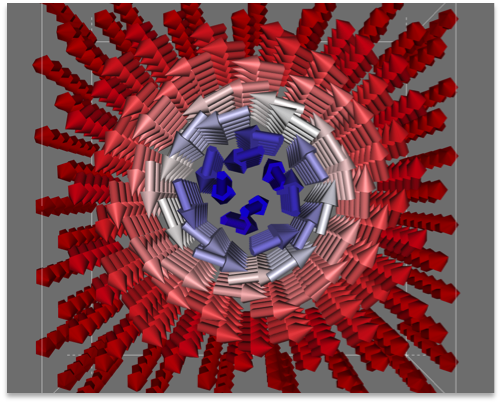
\includegraphics[width=.99\linewidth]{Figures/MnGe_skyrmion.png}
		  %\caption{}
		  \label{fig:sub1}
	\end{subfigure}%
	\begin{subfigure}{.5\textwidth}
		  \centering
		  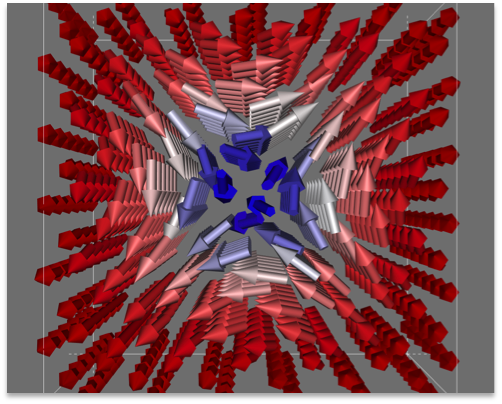
\includegraphics[width=.99\linewidth]{Figures/MnGe_antiskyrmion.png}
	          %\caption{}
                  \label{fig:sub2}
	\end{subfigure}
	\caption{Graphical representation of a Skyrmion (left) and an anti-skyrmion (right) 
	with atom magnetization pointing in positive (red) and negative (blue) z-direction. Results
	are obtained from a micromagnetic model with parameters for B20-MnGe
	taken from electronic structure calculations.}
	\label{fig:sd_results}
\end{figure}

Based on these simulations we also deem it
possible that textures even more exotic than skyrmions and anti-skyrmions as proposed in 
\cite{rybakov_new_2015},
can be stabilized in B20-MnGe.
\\
In the past few months, we have performed the
first KKRnano calculations for B20-MnGe on the HPC machines JUQUEEN,
JURECA and QPACE3. A 6x6x6 supercell of MnGe with 1728 atoms, has an
edge length of 3 nm and is small enough for routine calculations with our code. We do not 
expect the skyrmion lattice period, which we hope to find in DFT calculations, to be exactly the 
one observed in the experiments, so we plan to increase the size of the supercell to a 12x12x12
supercell with 13824 atoms and a length of 6 nm. If necessary, we can increase the size
to a 24x24x24 supercell with 110592 atoms \cite{brommel_juqueen_2017}.
\\
Our agenda is composed of the following sub-projects that we consider to be of importance
to a deeper understanding of helical textures in
B20-MnGe.

\subsubsection{Identification of non-trivial magnetic ground states in B20-MnGe}
The most important task by far connected to large-scale DFT calculations for MnGe is the search for
non-trivial magnetic ground states as opposed to trivial ones,
e.g. ferromagnetism or anti-ferromagnetism.
Here, our top priority is to simulate the 3q-state mentioned above. In addition, we plan
the simulation of single stable
skyrmions and anti-skyrmions. In particular, anti-skyrmions are of great interest as they
have seldom, if ever, been observed in any material.
%\\
%The calculations planned here are going to require much parameter tuning
%(e.g. supercell size) and testing to find
%suitable configurations and therefore
%\textbf{we consider an allocation of 20 million core hours as necessary for this sub-project.}
\subsubsection{Creation mechanisms leading to non-trivial magnetic states in B20-MnGe}
The identification of ground-state candidates is to be followed by an investigation of
mechanisms that lead to the formation of such ground-states. Our all-electron approach will allow 
us to exactly quantify the origin of differences in total energy and therefore give us strong hints
to what the system-inherent physics are driven by.
%\\
%\textbf{We estimate a need for 5 million core hours for this sub-project.}
\subsubsection{Investigation of Mn(1-x)Fe(x)Ge alloys}
Both B20-MnGe and B20-FeGe are chiral magnets exhibiting helical structures. While in
B20-MnGe a surprisingly short helical wavelength of 3-6 nm is observed \cite{tanigaki_real-space_2015},
a much larger one of
approx. 70 nm is seen in B20-FeGe \cite{lebech_magnetic_1989}. This huge difference has not yet been explained.
Our hypothesis is that it originates from fundamentally different effects, i.e. that
magnetic frustration dominates in B20-MnGe while in B20-FeGe the interplay between
isotropic exchange interaction and Dzyaloshinskii-Moriya interaction plays a major role.
\\
We plan to
simulate Mn(1-x)Fe(x)Ge alloys where the concentration of Mn and Fe is varied.
This work is going to help us solve the question of what is the fundamental difference in chiral magnetism
between
chiral magnetism in B20-MnGe and B20-FeGe.
%\\
%\textbf{15 million core hours are accounted for this sub-project.}

\subsubsection{Influence of impurities and defects in B20-MnGe}
B20-MnGe samples used to gather experimental data inevitably contain impurities and defects 
that may influence the magnetic properties of materials and thus play a crucial role
in the creation and stability of helical structures.
Much interesting research has already been done on the interplay of
skyrmions and impurities/defects for other structures
\cite{fert_skyrmions_2013,woo_observation_2016,jiang_direct_2016,crum_perpendicular_2015}.
We shall extend this research to B20-MnGe and
study the effect of impurities and point defects, e.g. oxygen interstitials.
%\\
%\textbf{10 million core hours are accounted for this sub-project.}

\subsection{Review Processes}
\textit{Has the underlying research project already successfully undergone a scientific review process? Is the project funded by public money?
If yes, please also provide information about the funding source
(e.g. State, BMWi, BMBF, DFG, EU, $\dots$)}

Projects based on KKRnano have been granted
granted substantial computing resources by several committees in the past years.
The code itself was awarded the High-Q club membership in 2014 which requires the ability to
efficiently utilize the entire 28-rack BlueGene/Q system installed in J\"ulich.
Our efforts are embedded in the framework of the recently approved DFG-funded
Priority Programme (SPP 2137)
that will become operational in 2018. 


%The development of the KKR method in general and of the code KKRnano in particular has been recognized 
%by the Board of Directors of Forschungszentrum J{\"u}lich as important work in the interest of 
%Forschungszentrum J{\"u}lich. The Board of Directors has supported the work by a Helmholtz professorship 
%for Prof. Peter Dederichs, as the third Jülich scientist to be honored with the award,
%after the Nobel Prize winner Prof. Peter Grünberg in 2007 and Prof. Siegfried Mantl in 2011. 
%The Board of Directors has also supported the work by authorizing the employment of Dr. Rudolf Zeller, 
%who reached the mandatory retirement age in Oct. 2014, as a part-time employee at least until Nov. 2017. 


\section{Numerical Methods and Algorithms} 
\rule{\textwidth}{0.4pt}\\
\textit{Describe the numerical methods and algorithms that you are planning to use, improve, or develop.}\\
 
\textit{(1 to 2 pages)}
\bigskip

Contrary to other DFT codes, which determine the Kohn-Sham orbitals by solving
the Kohn-Sham differential wave equation, in KKRnano the Green function for the Kohn-Sham
equation is obtained by solving an integral equation in real space. For the solution, space is divided
into non-overlapping cells around the atoms, and the calculations are separated into single-cell parts
where only the potential within the individual cell enters, and a large complex linear matrix equation for 
the matrix elements $G_{LL}^{nn'} (\epsilon)$ of the Green function $G(r, r , \epsilon)$:
\begin{equation}
	G_{LL'}^{nn'} (\epsilon) = G_{LL'}^{r,nn'} (\epsilon) + \sum_{n''} \sum_{L''}
	G_{LL''}^{r,nn''} (\epsilon) \sum_{L'''} \Delta t_{L'' L'''}^{n''} (\epsilon)
	G_{L'''L'}^{n''n'} (\epsilon)
	\label{eq:dyson_eq}
\end{equation}
In the following we refer to $\Delta t_{L'' L'''}^{n''} (\epsilon)$ as the $\Delta t$-matrices and
$G_{LL''}^{r,nn''} (\epsilon)$ as the reference Green functions. We refer the reader to the existing
literature for more details \cite{zeller_towards_2008}.
\\
The given problem is identical to solving a complex linear matrix equation of the form
\begin{equation}
	\matr{A} \vec{x} = \vec{b}
\end{equation}
As is well known this problem scales as $O(N^3)$, where $N$ denotes the dimension of the $N \times N$
matrix $\matr{A}$. Standard solving schemes therefore severely limit the system size that can
be calculated.
However, by choosing a reference system of repulsive potentials
$\matr{A}$ can be made sparse and this can again be exploited
by using customized iterative algorithms for solving linear sparse matrix equations.
Our method uses the transpose free quasi minimal residual (TFQMR) algorithm \cite{freund_qmr:_1991}
which enables us to achieve $O(N^2)$ scaling. 
Convergence of the TFQMR iterations is achieved by working in the complex energy plane. Both concepts,
the repulsive reference system and application of complex energy, were
introduced by us into the KKR method \cite{zeller_application_1982,zeller_theory_1995}
and are used worldwide for many years. 
By truncating inter-atomic interactions above a certain distance, an $O(N)$ scaling 
behavior can be realized, and this feature should be used in any calculation involving more than 1000 atoms.
In most applications the TFQMR solver accounts for more than 70 \% of the computational work.
\\
For super-large-scale calculations (above 100000 atoms) the electrostatics solver begins
to require an amount of computing resources that is not negligible anymore. 
The electrostatic problem is given in terms of a Poisson equation that connects electric field and potential. 
Solving this equation scales quadratically with system size. 


\section{Computer Resources}
\rule{\textwidth}{0.4pt}\\
\subsection{Code performance and workflow}
%\textit{Describe the codes, packages or libraries that you need to undertake the project, and how these will enable the research to be achieved. Include for \textbf{each code to be used} information about}
%\begin{itshape}
%\begin{itemize}\setlength{\itemsep}{-2pt}
%  \item Which code will be used
%  \item How is the code parallelized (pure MPI, mixed MPI/OpenMP, Pthreads, CUDA, etc.)
%  \item The amount of memory necessary (per core, per node and in total)
%  \item Scaling plots \textbf{and} tables with speedup results for runs with typical, parameter sets, problem size, and I/O \textbf{of the planned project} (no general benchmark results are accepted)
%  \item Describe architecture, machine/system name, and problem size used for the scaling plots
%  \item Current job profile (independent jobs, chained jobs, workflow, etc.)
%\end{itemize}
%\end{itshape}

The natural parallelization strategy in KKRnano is domain decomposition with a simple 
matching between atomic cells and processors. Both the single scattering part of the 
calculations and the iterative solution of \cref{eq:dyson_eq} can be done separately for each cell. 
Communication between the processors is required to distribute the
$\Delta t$-matrices and the 
reference Green function matrix
before \cref{eq:dyson_eq} is solved and because density information
must be distributed to obtain the electrostatic potential for the next density functional
self-consistency step. KKRnano is also parallelized over the energy points $\epsilon$ and 
the two spin directions so that more than one MPI process per atom can be utilized.
On the other hand, it is also possible to map several atoms to one MPI process so that
systems with several thousand atoms can also be investigated if only a few hundred
processors are available, but with associated longer wall-clock runtimes.
\\
For an efficient use of computers featuring symmetric multiprocessing (SMP) KKRnano contains OpenMP directives
in the most time consuming parts, so that e.g. on JUQUEEN calculations can be performed with combinations 
ranging from 1 MPI task and 64 threads to 64 MPI tasks and 1 thread per node. Weak-scaling data
for different combinations
obtained on JUQUEEN is depicted in \Cref{fig:total_runtimes}.
\begin{figure}[h]
\begin{center}
 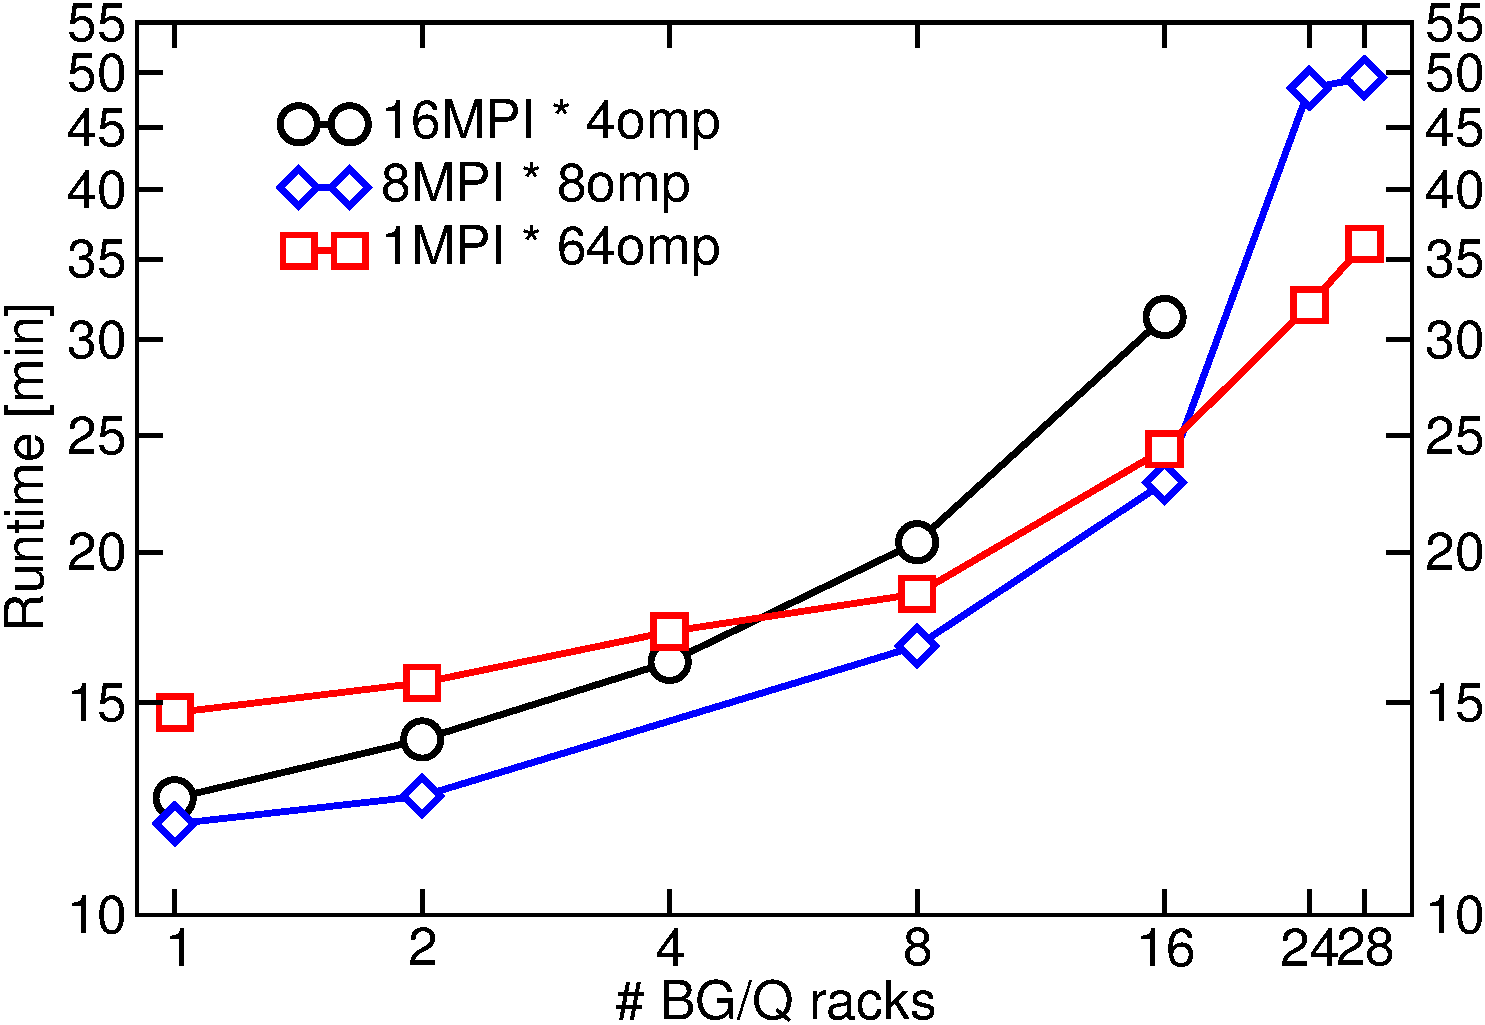
\includegraphics[scale=0.45]{Figures/total_runtimes.pdf}
\end{center}
\caption{Runtime of one self-consistent iteration with KKRnano 
	on IBM BlueGene/Q at Forschungszentrum J{\"u}lich.
	This data was obtained with a problem size ranging from 8192 atoms (1 rack) to 229376 atoms (28 racks).
	Different distribution of MPI tasks (MPI) and OpenMP threads (omp) leads to slightly different runtimes.}
\label{fig:total_runtimes}
\end{figure}
For these performance tests MnGe supercells
with 8192 atoms (1 rack) to 229376 atoms (28 racks/full machine) were used.
In order to achieve linear scaling in the TFQMR solver the calculations were 
done by setting the interaction range described by truncation of the Green function to include 
1308 atoms around each considered site.
\Cref{fig:tfqmr_es_times} provides a scaling analysis of the TFQMR and electrostatics solver.
\begin{figure}[h]
\begin{center}
 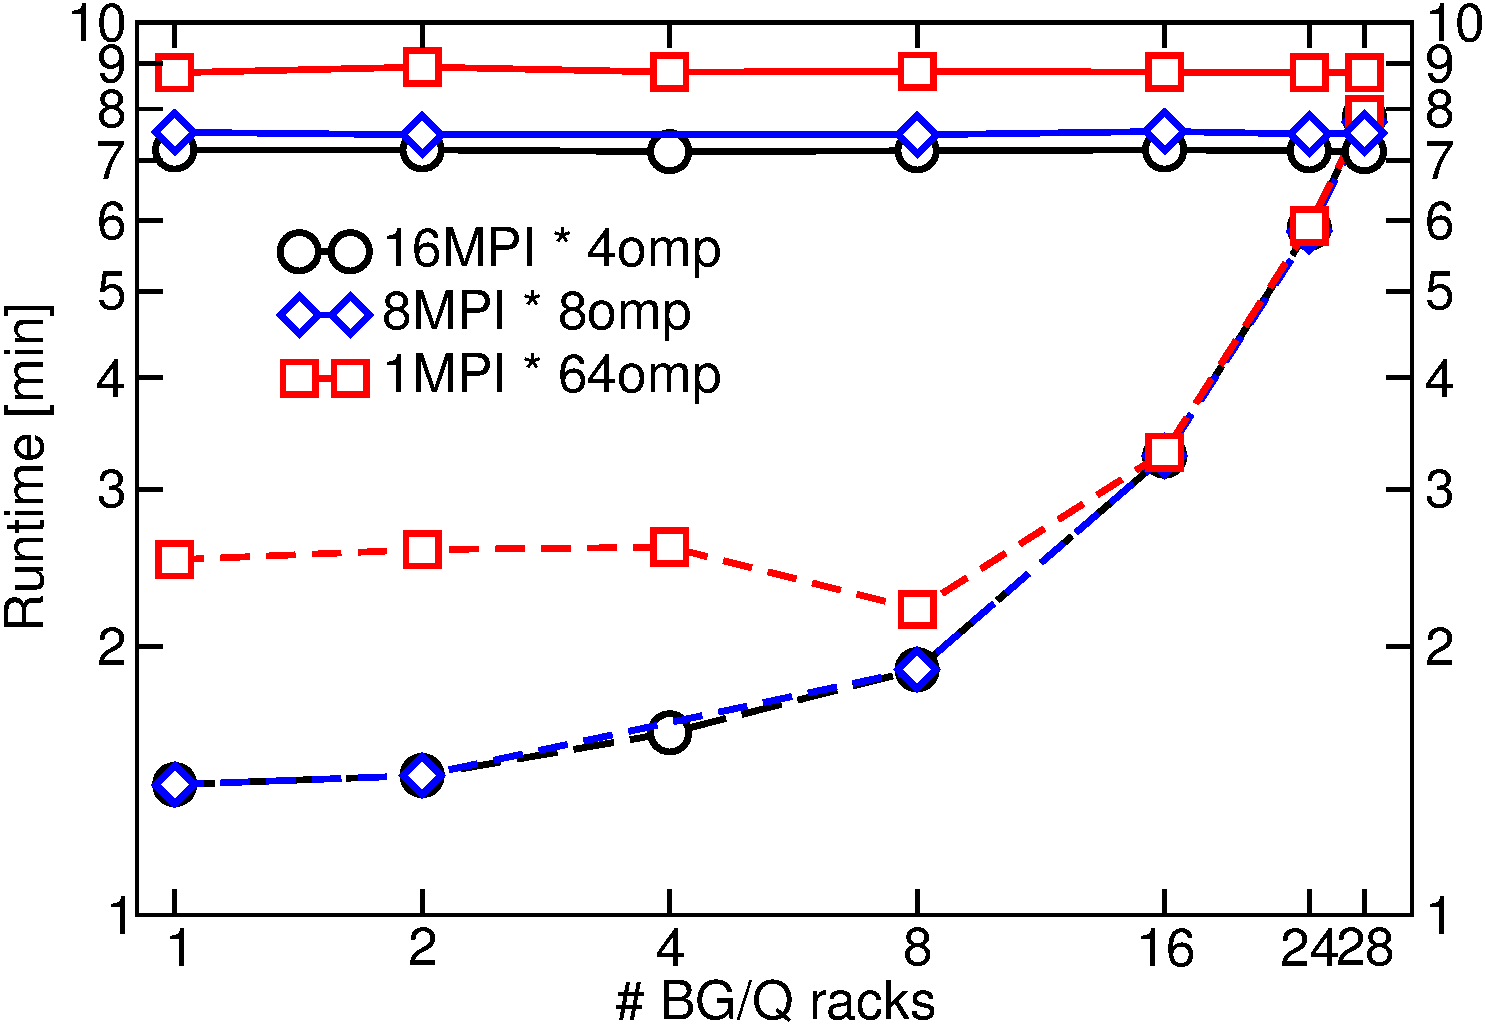
\includegraphics[scale=0.45]{Figures/combinedtfqmrelectrostatics.pdf}
\end{center}
\caption{Time per iteration spent in the TFQMR solver (solid lines) 
	and in the electrostatics solver (dashed lines) for the calculations depicted in
	\Cref{fig:total_runtimes}.}
\label{fig:tfqmr_es_times}
\end{figure}
It shows 
a constant runtime of the TFQMR solver but also that the runtime of the electrostatics solver becomes
more and more significant when calculations are done for more than 65536 atoms (8 racks). 
The standard system sizes we are aiming
for with this project proposal will, however, be smaller than that.
The small discrepancy between \Cref{fig:total_runtimes} and \Cref{fig:tfqmr_es_times} with regards to linear
scaling can be mainly attributed to Fortran direct-access I/O which does not scale well on a GPFS file system.
The implementation of a more suitable I/O library (e.g., MPI I/O or SIONlib) is likely to solve this issue.
In terms of memory consumption it could be observed that the 1GB/core ratio on JUQUEEN is not exceeded.
Additionally, test runs on Hazel Hen showed that the memory provided per node is sufficient for the calculations
planned.
\\
KKRnano jobs are launched as independent jobs requiring a short (less than 60 seconds) serial 'prepare'-step on
the head node
before launching the parallel large-scale calculation. All post-processing will be
performed on local computers.

%{\it \textbf{Important:} please take into account the corresponding technical guidelines and requirements (e.g. required minimal code scalability, memory restictions, etc.) of the machine you have chosen!}\\

%\textit{Here we give an example table and plot for presenting scaling and performance information.}

%\begin{table}[H]
%\caption{\label{tab_scaling} Scaling behavior of {\tt $<$code$>$} on {\tt $<$architecture and system$>$} at {\tt $<$location$>$}. This test was performed with $5\cdot 10^6$ particles, absolute timings per timestep (s) and relative speedup normalized to 1024 cores are given.}
%\begin{center} 
%\setlength{\tabcolsep}{10pt}
%\renewcommand{\arraystretch}{1.2}
% \begin{tabular}{lcccc}
% \#cores  & absolute timing (s) & speedup  & Performance per core [MFLOP/s]\\
%\hline
%1024     & 189.6                        & 1.0000   & 600 \\
%2048     & \phantom{1}99.0      & 1.9154   & 576 \\
%4096     & \phantom{1}55.6      & 3.4088   & 511 \\
%8192     & \phantom{1}30.8      & 6.1376   & 460 \\

%\end{tabular}
%\end{center}
%\end{table}


%\begin{table}[h!]
%	\caption{Scaling behaviour of KKRnano on JUQUEEN at Forschungszentrum J{\"u}lich. 
%		Total runtime (Total), tfQMR solver runtime (tfQMR) and electrostatics solver runtime (ES)
%		    in weak scaling measurement series employing moderate OpenMP parallelization
%		      with $16$ MPI ranks per node and $4$ threads per process. 
%		        Runtimes are given in seconds. (t) indicates the tuned version where final I/O is omitted.}
%			\begin{center}
%				\begin{tabular}{|c|r|r|r|r|r|r|}
%					\hline
%					 Supercell               & bg\_size & MPI ranks &   Threads &    Total & tfQMR &  ES \\
%					\hline\hline
%					$16 \times  8 \times  8$ &  1,024   &  16,384   &    65,536 &      750 &   432 &  84 \\
%					$16 \times 16 \times  8$ &  2,048   &  32,768   &   131,072 &      839 &   432 &  86 \\
%					$16 \times 16 \times 16$ &  4,096   &  65,536   &   262,144 &      973 &   430 &  96 \\
%					$32 \times 16 \times 16$ &  8,192   & 131,072   &   524,288 &     1223 &   431 & 113 \\
%					$32 \times 32 \times 16$ & 16,384   & 262,144   & 1,048,576 &     1880 &   432 & 196 \\
%					$32 \times 32 \times 24$ & 24,576   & 393,216   & 1,572,864 & (t) 1077 &   431 & 353 \\
%					$32 \times 32 \times 28$ & 28,672   & 458,752   & 1,835,008 & (t) 1210 &   430 & 470 \\
%					\hline
%				\end{tabular}
%			\end{center}
%			\label{kkrnano:mnge_weakscaling_moderateomp}
%		\end{table}





\textit{(1 to 2 pages)}
\newpage
\subsection{Justification of resources requested}
\label{sec:just}
%\textit{Outline the amount of resources you request for the current granting period, structured in sub-projects, if applicable. This should include information such as}
%\begin{itshape}
%\begin{itemize}\setlength{\itemsep}{-2pt}
%    \item Type of run (e.g. pre- /post-processing run, production run, visualization, etc.)

%    \item Problem size for planned runs (e.g. \# particles or the like)
%    \item Number of runs planned
%    \item Number of steps per run
%    \item Wall-clock time per run
%    \item Number of cores/GPUs used per run
%    \item Total amount of requested computing time (core-hours and/or GPU-hours, if applicable)
%    \item Resources for data analytics, if applicable
%\end{itemize}
%\end{itshape}

We plan to do pure production runs that feature different non-trivial magnetic textures, such as skyrmions.
Each run consists of typically about 100 self-consistent iterations that are needed to converge
the electronic density. Our current setup requires approximately 1000 s per iteration depending on the desired
accuracy. We emphasize that such calculations depend on several tunable parameters, e.g. number of
k-points, cutoff radii and atomic positions, and it is essential to check results with different parameter
settings in order to ensure that physical interpretations are valid and reproducible. 
%With the \textbf{requested amount of 50 million core hours} (approx $1.8 \times 10^{11}$ core-s)
%we are able to do roughly 1000 independent calculations with
%the smallest setup featuring a unit cell of 1728 atoms:
%\begin{equation}
%	n_{\text{calculations}} = \frac{1.8 \times 10^{11} }{ 1000 \times 100 \times 1728} \approx 1000 
%\end{equation}
%For the larger calculations computational needs increase linearly, e.g. a setup of
%13824 atoms allows for 125 full calculations given 50 million core hours on Hazel Hen.
Note that
experimental data suggests that the 3q-state in B20-MnGe can be stabilized on a length scale 
of 3-6 nm which corresponds to a supercell size of
1728 to 13824 atoms.

%\textit{This information should take the form of a table like the example table shown below. Please, specify the requested time in appropriate units, preferred units are core hours (core-h) and GPU-hours.}\\


\bigskip

\begin{tabular}{llcccccc} \hline\hline
  Sub-project & 
  Type &
  Problem & 
  \# runs & 
  \# steps/ & 
  Wall time/ & 
  \# cores/ & 
  Total \\
  &
  of run &
  size  &
  &
  run &
  step [hours] &
  run &
  [core-h] \\
 \hline\hline
  Sub-proj. 1 & 
  standard &
  1728-13824 & 
  50-400 & 
  100 &
  0.28 &
  1728-13824 &
  20 mio. \\
     &
     &
    atoms & 
     & 
     &
     &
     &
     \\
  Sub-proj. 2 & 
  DOS/XC &
  1728-13824 & 
  40-300 & 
  1 &
  10.0 &
  1728-13824 &
  5 mio. \\
     &
     &
    atoms & 
     & 
     &
     &
     &
     \\
  Sub-proj. 3 & 
  standard &
  1728-13824 & 
  40-300 & 
  100 &
  0.28 &
  1728-13824 &
  15 mio. \\
     &
     &
    atoms & 
     & 
     &
     &
     &
     \\
  Sub-proj. 4 & 
  standard &
  1728-13824 & 
  25-200 & 
  100 &
  0.28 &
  1728-13824 &
  10 mio. \\
     &
     &
    atoms & 
     & 
     &
     &
     &
     \\



$\cdots$ &\multicolumn{7}{c}{$\cdots$}\\
\hline\hline
TOTAL & & & & & & & 50 mio. \\
\end{tabular}
\bigskip

\textit{(0.5 to 1 page)}

\subsubsection{Sub-project 1: Identification of non-trivial magnetic ground states in B20-MnGe}
The crucial parameter for identifying non-trivial magnetic ground states is the
supercell needed to host the magnetic texture.
A 6x6x6 supercell (1728 atoms) differs from the size of the 8x8x8 supercell (13824 atoms)
by a factor of 8 in required computing resources. A allocation of 20 million core-hs would allow
us to conduct 50 to 400 complete runs depending on the supercell size.
This does not mean that 50 to 400 different textures can be simulated, but
we expect to carry out approximately 10 runs per texture since consistency checks with regards to 
small changes of lattice constant, exchange-correlation functional etc., must be made.

\subsubsection{Sub-project 2: Creation mechanisms leading to non-trivial magnetic states in B20-MnGe}
After having identified interesting states it is essential to investigate the underlying creation mechanisms.
To do this we need to extend our calculations from merely total energy calculations to 
a deeper analysis where we rely, e.g. on the electronic density of states (DOS) or on the extraction
of magnetic exchange coupling (XC) constants. 
Such calculations require only one iteration using an already self-consistently converged potential, but
this iteration takes approx. 10 hours.
%Such calculations should only be done for a handful of promising setups as they demand a walltime that is
%roughly ten times larger than that of a 'normal' calculation.

\subsubsection{Sub-project 3: Investigation of Mn$(1-x)$Fe$(x)$Ge alloys}
In this sub-project we plan to tune the concentration parameter $x$ in steps of
$\Delta x = 0.1$ and then perform calculations for each resulting alloy. This
sub-project will start after investigations of sub-project 1 are finished
and magnetic textures of interest have been identified.
Textures of specific interest can then be simulated in Mn$(1-x)$Fe$(x)$Ge alloys.
Because these calculations must be done for each alloy we expect
it to be computationally almost as intensive as sub-project 1.

\subsubsection{Sub-project 4: Influence of impurities and defects in B20-MnGe}
We request an additional 10 mio. core-hs for the study of impurities and defects in MnGe,
where it is necessary to converge the system self-consistently for each
deviation from pure B20-MnGe. Approximately 100 iterations need
to be performed each time.




\section{Resource Management and Work Schedule}
\rule{\textwidth}{0.4pt}\\
%\subsection{Resource management}
%\textit{Describe how you intend to manage the resources you have requested. This should include a description of the methods you will deploy to monitor progress of the project and how project results are documented.}\\

\textit{(0.5 to 1 page)}

%\subsection{Work schedule}
%\textit{Please, provide a short work schedule, structured in sub-projects, if applicable. Include a table and/or Gantt chart.}

%\subsubsection{Sub-project 1}
%\textit{...}

%\subsubsection{Sub-project 2}
%\textit{...}\\

The progress of the work concerned with the development and the application of KKRnano
is discussed in regular bi-weekly strategy meetings of the project team.
The code development and the protocols of the strategy meetings are documented
using the Trac system at URL https://trac.version.fz-juelich.de/KKRnano so
that all changes to the code and all experience with its use are readily available.


\bigskip
%\textit{Example for a Gantt chart:}
%\begin{figure}[H]
%\begin{flushleft}
% \includegraphics[scale=0.82]{Figures/gantt_chart.jpg}
%\end{flushleft}
% \caption{\label{fig_workschedule}Work schedule for the project.}
%\end{figure}

\section{Key Personnel and Experience}
\rule{\textwidth}{0.4pt}\\
\textit{Give a short introduction of the key persons involved in the project and their experience (max 3 persons).}\\

\textit{(half a page)}

Prof. Stefan Bl{\"u}gel is...
His publication record can be found on ORCiD [\url{https://orcid.org}] (id: 0000-0001-9987-4733) 
and Researcher ID
[\url{http://www.researcherid.com}] (id: J-8323-2013).
\\
Marcel Bornemann is a PhD student who has
detailed knowledge of the computer code KKRnano and of the principles of writing modern code. 
He implemented important enhancements in KKRnano such as the extension to non-collinear
magnetism including relativistic effects.
\\
Dr. Sergii Grytsiuk is...
\\
Dr. Roman Kovacik is...
\\
Dr. Rudolf Zeller has been working in the field of density-functional calculations for more than 40 years. 
He is the main developer of the full-potential KKR programs, including KKRnano, 
which are now used in J{\"u}lich and several other places in Germany.
His publication record can be found on ORCiD [\url{https://orcid.org}] (id: 0000-0002-9462-2649) 
and Researcher ID
[\url{http://www.researcherid.com}] (id: K-7094-2013).
\\
Dr. Phivos Mavropoulos is a Principal Investigator at the Institute for Advanced Simulation—Quantum
Theory of Materials, Forschungszentrum J\"ulich.
He has been working on the development and application of KKR-based codes for 20 years. 
His expertise lies in density-functional-based calculations of magnetic and transport
properties of metallic and insulating systems, including complex problems as non-collinear magnetism, 
tunnel junctions, impurities and impurity scattering, magnetic interactions and phase transition temperatures.
His publication record can be found on ORCiD [\url{https://orcid.org}] (id: 0000-0002-0205-8025) 
and Researcher ID
[\url{http://www.researcherid.com}] (id: H-6189-2013).
\\
Dr. Paul F. Baumeister is...

\newpage

\bibliography{My_Library}

%\section{Bibliographic References}
%\rule{\textwidth}{0.4pt}\\
%\textit{Provide recent/most important bibliographic references that are relevant to the project.}\\

\bigskip
\begin{flushright}
{\tiny V1.3-2016JUN07}
\end{flushright}
\end{document}
